\section{後処理と描画} \label{sec:ideal_exp_net2g}
%------------------------------------------------------
ここでは、計算結果を描画するための後処理について説明する。本書のチュートリアルでは、
NetCDF形式の分散ファイルを1つのファイルにまとめ、ユーザが解析しやすいDirect-Accessの
単純バイナリ形式(\grads 形式)に変換する方法を説明する。
%GPhys/Ruby-DCLを使うと
%分割ファイルのまま直接描画することができるが、この方法については\ref{sec:quicklook}節を
%参照してもらいたい。

まず、\ref{sec:source_net2g}節でコンパイルした後処理ツール\verb|net2g|へリンクを張る。
\begin{verbatim}
  $ ln -s ../../../util/netcdf2grads_h/net2g  ./
\end{verbatim}
%もし、ここで説明するディレクトリとは異なる場所で実行している場合は、
%リンクを張る時のディレクトリ指定に注意すること。

\verb|net2g| も実行方法は基本的にSCALE本体と同じである。
\begin{verbatim}
  $ mpirun  -n  [プロセス数]  ./net2g  [設定ファイル]
\end{verbatim}
net2g専用の \verb|net2g_R20kmDX500m.conf|を設定ファイルとして与えて、
次のように実行する。
\begin{verbatim}
  $ mpirun  -n  2  ./net2g  net2g_R20kmDX500m.conf
\end{verbatim}
エラーメッセージがなく、下記のメッセージだけが標準出力へ表示されていれば正常に変換完了である。\\

\noindent {\gt
\fbox{
\begin{tabularx}{150mm}{l}
\verb|+++ MPI COMM: Corrective Finalize| \\
\end{tabularx}
}}\\

\noindent net2gの実行にあたっては、SCALE本体の実行時に使用したMPIプロセス数と同じか、
その約数のプロセス数を用いて実行しなければならない。
%HDDの読み書き速度に依存するが、本書の必要要件にあった計算機であれば2分程度で計算が終わる。
この実行によって、下記6つのファイルが、実行ディレクトリ下に作成される。
\begin{alltt}
  QHYD_d01z-3d.ctl
  QHYD_d01z-3d.grd
  U_d01z-3d.ctl
  U_d01z-3d.grd
  W_d01z-3d.ctl
  W_d01z-3d.grd
\end{alltt}
これらのファイルはぞれぞれ、分割ファイルを1つにまとめ、
U(水平風東西成分)、W(鉛直風)、QHYD(全凝結物の質量比)の変数について
ダイレクトアクセスの単純バイナリ形式(\grads 形式)に
変換したgrdファイルと\grads に読み込ませるためのctlファイルである。

計算がうまくいっているかを確認するため、\grads スクリプト \verb|checkfig_ideal.gs|
を使って作図する。なお、\grads のバージョンによっては文法が異なるので、
Warningが出る場合は適宜\grads スクリプトを変更する。
\begin{verbatim}
  $ grads -blc checkfig_ideal.gs
\end{verbatim}
作図が成功すると、下記の図が生成される。
\begin{verbatim}
   ideal_QHYD.png
   ideal_W.png
\end{verbatim}
計算と変換が成功していれば、図\ref{fig_ideal}と同じ図が描画される。

\begin{figure}[t]
\begin{center}
  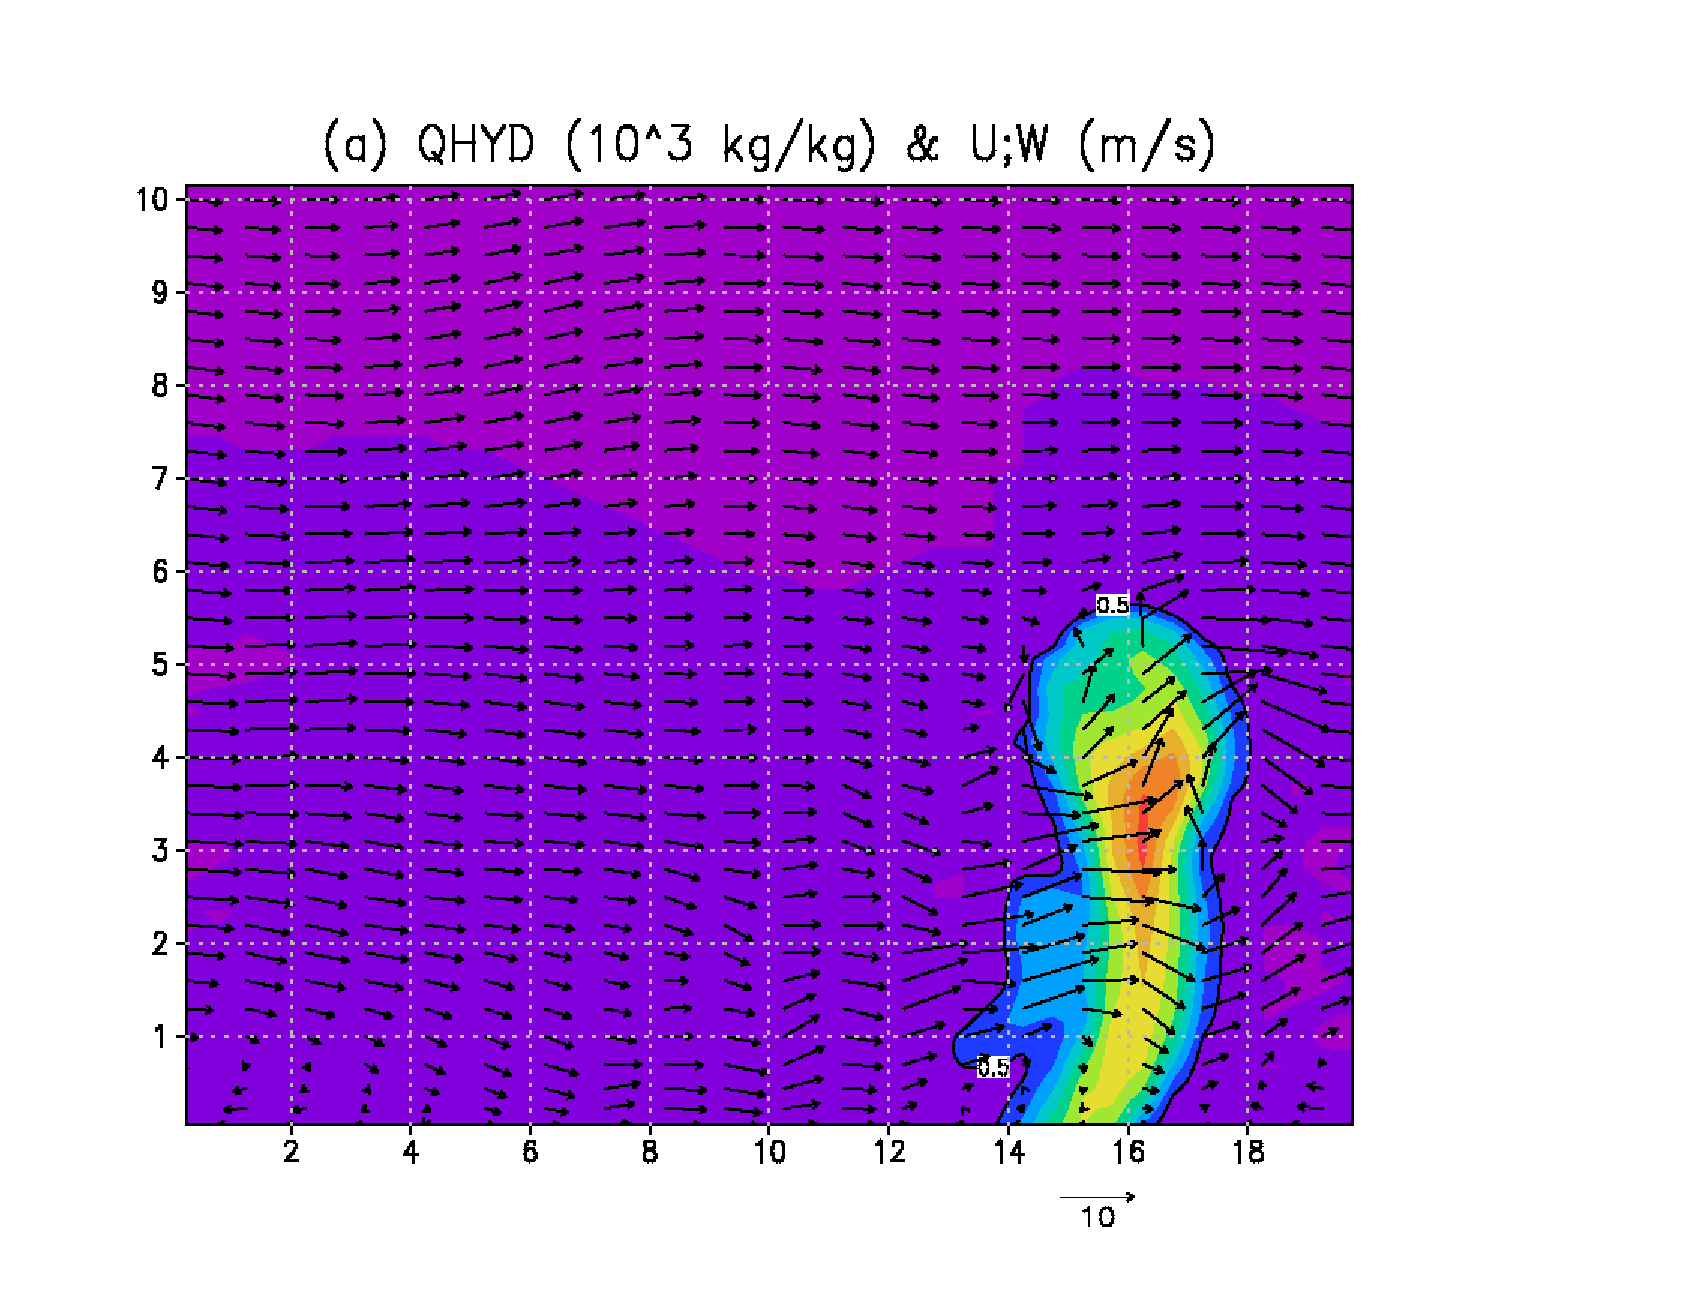
\includegraphics[width=0.7\hsize]{./figure/ideal_qhyd.eps}\\
  \includegraphics[width=0.7\hsize]{./figure/ideal_W.eps}\\
  \caption{積分開始後 1200 sec (20 minute) のY=750mにおける東西-鉛直断面図;
           (a)のカラーシェードは全質量に対する凝結物の質量比、
           (b)は鉛直速度をそれぞれ示す。ベクトルは東西-鉛直断面内の風の流れを表す。}
  \label{fig_ideal}
\end{center}
\end{figure}


他の変数についてもバイナリデータに変換したい場合には、
\verb|net2g_R20kmDX500m.conf|の\namelist{VARI}の\nmitem{VNAME} に必要な変数を追加すればよい。\\

\noindent {\small {\gt
\ovalbox{
\begin{tabularx}{150mm}{l}
\verb|&VARI|\\
\verb| VNAME       = "U","W","QHYD"|\\
\verb|/|\\
\end{tabularx}
}}}\\

\noindent
historyファイルに出力されている変数は、{\netcdf} の\verb|ncdump| などを
使えば簡単に調べることができる。net2gの詳しい使用方法は、\ref{sec:net2g}を参照してほしい。




